\chapter{Statistical Simulation for Spatial Sampling}

The angle increment was derived in section \ref{sec:spasa} and is presented in equation \ref{eq:angle}. To find a compromise between measurement speed and accuracy a perfect trade off in terms of aliasing error has to be found. For a perfect adjustment of the measurement uncertainty, dependent on the \ac{SF}, the measurement error shall be independent of the devices' aperture.

\section{Implementation}

The simulation is similar to section \ref{sec:spasa}, carried out using the \ac{AF}, however with a two-dimensional rectangular $\sfrac{\lambda}{2}$-element spacing array. This brings the advantage that the array size can easily be adjusted. The \ac{FF}-pattern is computed with the Matlab\texttrademark{} class \textit{phased.URA}.
The class can be parameterized with a steering vector, consistent of an azimuth and an elevation angle, to specify which direction the main beam of the array is facing, the array's size, the properties of the radiating elements, in this case isotropic radiators, and the element spacing, in this case $\sfrac{\lambda}{2}$.
The sampling of the \ac{FF}-pattern is accomplished by the included \textit{pattern(...)} method.\\
This simulation is mainly developed for \acp{CSSG} and the angle increment is computed by equation \ref{eq:angle}. With the number of elements in $z$ direction $N_z$ and the number of elements in $y$ direction $N_y$ the radii $r_s$ and $r_c$ can be calculated as

\begin{equation}
2r_s = \sqrt{\left(N_y-1\right)^2+\left(N_z-1\right)^2}\cdot\frac{\lambda}{2},\quad 2r_c=\left(N_y-1\right)\cdot\frac{\lambda}{2},
\end{equation}

resulting in an angle increment of

\begin{equation}
\Delta\Theta^\prime = \frac{\text{SF}\cdot\text{CrefA}\left(\sfrac{2r_s}{\lambda}\right)\cdot 2}{\sqrt{\left(N_y-1\right)^2+\left(N_z-1\right)^2}}\ ,\quad\Delta\Phi^\prime = \frac{\text{SF}\cdot\text{CrefA}\left(\sfrac{2r_c}{\lambda}\right)\cdot 2}{\left(N_y-1\right)}\,.
\end{equation}

Whereby \ac{CrefA} is a function of diameter in wavelength, as shown in fig. \ref{fig:crefa}. The number of points on each longitude half circle $N_\Theta$ and on each latitude circle $N_\Phi$ is computed and rounded up

\begin{equation}
N_\Theta = \bigg\lceil\frac{\pi}{\Delta\Theta^\prime}\bigg\rceil ; \quad N_\Phi^\prime = \bigg\lceil\frac{2\pi}{\Delta\Phi^\prime}\bigg\rceil\,.
\end{equation}

For sparser sampling at the poles, the \ac{CTF} with a value range of $\text{CTF}=\left[0,1\right]$ is introduced to gain Theta dependent azimuth step size

\begin{equation}
N_\Phi\left(\Theta\right) = \bigg\lceil\frac{2\pi}{\Delta\Phi^\prime}\left(1-\text{CTF}+\text{CTF}\cdot\cos\right(\Theta\left)\right)\bigg\rceil\,.
\end{equation}

If it turns out that the \ac{CTF} is independent of the resulting uncertainty, then $\text{CTF}=1$ can be chosen and n order to reduce the number of measurement samples. For easier computation $N_\Phi\left(\Theta\right)$ is round to 

\begin{equation}
N_\text{round} = \bigg\lceil \frac{N_\Phi^\prime}{k} \bigg\rceil, \ k \in \mathbb{N}
\end{equation}

and not to the greater integer. So that the angle increment is

\begin{equation}
\Delta\Theta = \frac{\pi}{N_\Theta} , \quad \Delta\Phi\left(\Theta\right) = \frac{2\pi}{N_\Phi\left(\Theta\right)}\,.
\end{equation}

The advantage of using the integers in $N_\text{round}$ instead of rounding to the next integer is, that the \ac{CSSG} can be sampled without \ac{CTF} and the theta dependent phi can be simulated by discarding every $k^\text{th}$ value in each azimuth circle.

\begin{figure}
  \centering
  \subfigure[PDF]{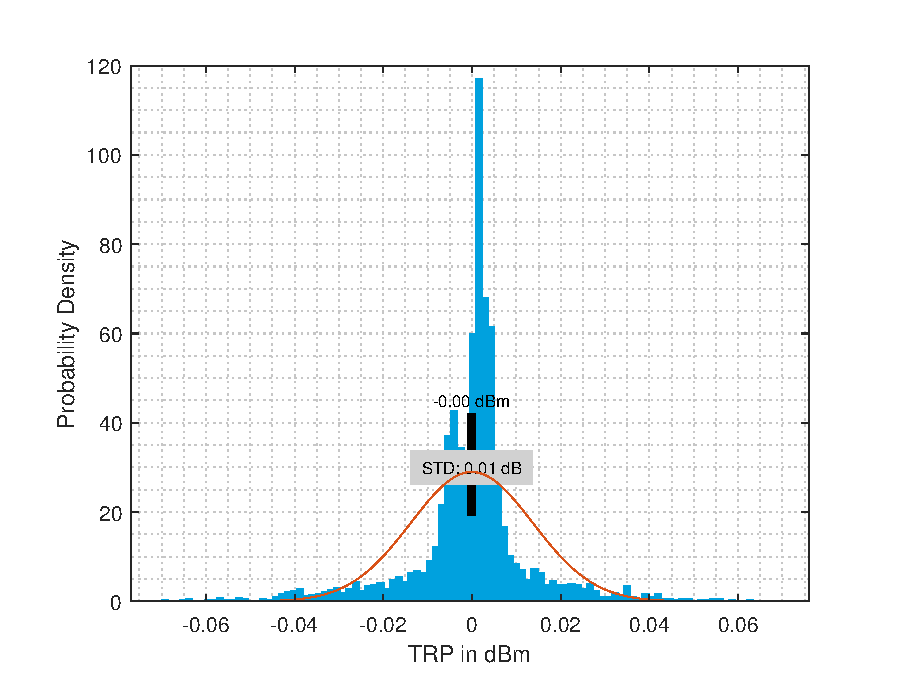
\includegraphics[width=0.49\textwidth]{Matlab/PDF_6-18_SF1.eps}}
  \centering
  \subfigure[CDF]{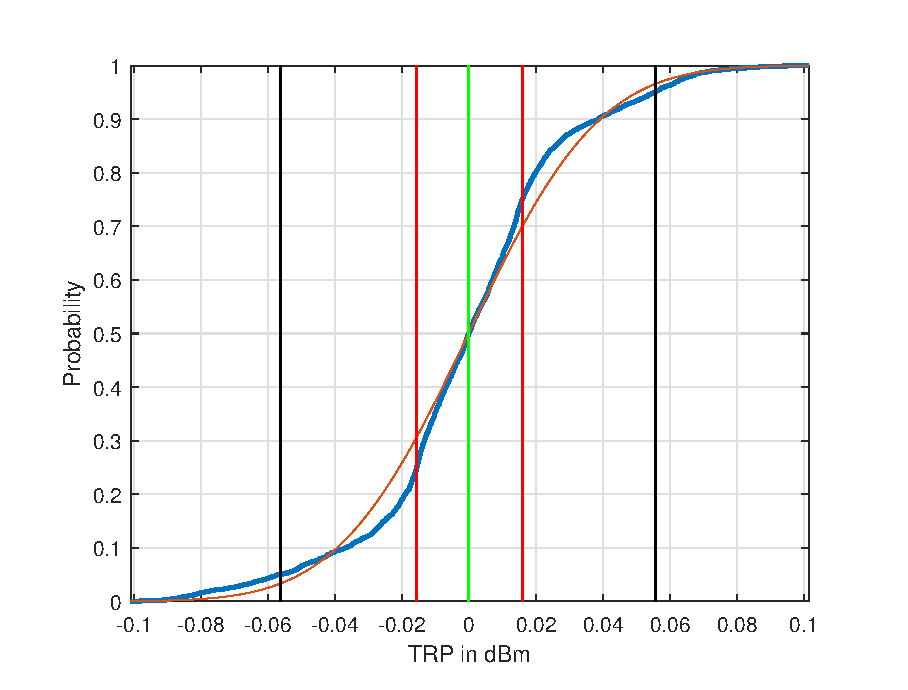
\includegraphics[width=0.49\textwidth]{{Matlab/CDF_6-18_SF1.eps}}}
\caption{4000 random steering vectors, $\text{SF}=1$, 6x18-Array}
\label{fig:rands}
\end{figure}

There are four input parameters: First the \ac{SF}, second the \ac{CTF} and third and fourth the elements of the array in $y$ and $z$ direction. Every set of parameters is simulated with $N=4000$ samples using random steering vectors. The azimuth steering is uniformly distributed within $-\pi$ to $\pi$. In elevation, a random variable is generated with a \ac{CDF} of \ac{CC} coefficients from $-\sfrac{\pi}{2}$ to $\sfrac{\pi}{2}$ by projecting uniformly distributed random numbers. This results in an uniformly distributed main beam direction over the spheres' surface. For every set of parameters the third step is iterated $N$ times:

\begin{enumerate}
\item Generate $N$ steering vectors.
\item Derive a \ac{CSSG}.
\item Compute the \ac{TRP}:
\begin{enumerate}
\item Generate an antenna pattern using a random steering vector. A sample for that is depicted in fig. \ref{fig:randp}.
\item Sample the antenna pattern with the derived grid.
\item Discard samples dependent on the \ac{CTF}.
\item Compute a \ac{TRP} using the \ac{CC}-quadrature.
\end{enumerate}
\end{enumerate}

A histogram and the resulting \ac{CDF} for one parameter set is plotted in fig. \ref{fig:rands} (a) and (b). In both diagrams additionally the \ac{PDF}, respectively \ac{CDF} of the normal distribution is plotted in orange. Because the normal distribution is not an accurate metric for the underlying distribution, the $\SI{90}{\percent}$ \ac{IQR}, from the $\SI{5}{\percent}$ quantile to the $\SI{95}{\percent}$ quantile, is used to describe the scattering. In fig. \ref{fig:rands} (b) the black lines are the $\SI{5}{\percent}$- and $\SI{95}{\percent}$- quantiles, the red lines the $\SI{25}{\percent}$- and $\SI{75}{\percent}$- quantiles and the mean is the green line.\\
The statistical experimental design is based on a D-optimal design dependent on the parameter matrix

\begin{equation}
X = \begin{bmatrix}
1 & \text{SF}_1 & \text{SF}_1^2 & \text{CTF}_1 & N_{y,1} & N_{z,1} & N_{y,1}N_{z,1}\\
\vdots & \vdots & \vdots & \vdots & \vdots & \vdots & \vdots\\
1 & \text{SF}_N & \text{SF}_N^2 & \text{CTF}_N & N_{y,N} & N_{z,N} & N_{y,N}N_{z,N}
\end{bmatrix}
\label{eq:parammatrix}
\end{equation}

with $M=7$ parameters. The D-optimal design is used because out of other documents e.g. \cite{2018arXiv180310993F} a coarse assumption to the significant parameters can be derived and thereby not every interaction needs to be tested. It is assumed that the \ac{SF} has also a quadratic dependency and that the linear interactions between the number of elements is significant. Therefore, a minimum number of samples is $N_\text{min}=1.5\cdot\left(M+1\right)=12$ \cite{dffs}. So a statistical experimental design can be derived using the Matlab\texttrademark{} \textit{cordexch(...)}-function with the input of the potency matrix of the regression

\begin{equation}
P = \begin{bmatrix}
0 & 0 & 0 & 0\\
1 & 0 & 0 & 0\\
2 & 0 & 0 & 0\\
0 & 1 & 0 & 0\\
0 & 0 & 1 & 0\\
0 & 0 & 0 & 1\\
0 & 0 & 1 & 1
\end{bmatrix},
\end{equation}

comparing the parameter matrix in equation \ref{eq:parammatrix}. With that the experimental design is derivable as 

\begin{equation}
X^\prime = \begin{bmatrix}
1&1&1&-1&1&-1&-1\\
1&1&1&1&-1&1&-1\\
1&1&1&1&-1&-1&1\\
1&0&0&-1&-1&-1&1\\
1&-1&1&-1&-1&-1&1\\
1&-1&1&-1&1&1&1\\
1&-1&1&1&-1&1&-1\\
1&-1&1&1&-1&-1&1\\
1&1&1&1&1&1&1\\
1&0&0&1&1&1&1\\
1&1&1&-1&1&1&1\\
1&-1&1&-1&-1&1&-1\\
1&0&0&-1&-1&1&-1\\
1&-1&1&1&1&-1&-1\\
1&1&1&-1&1&-1&-1\\
1&0&0&1&1&-1&-1
\end{bmatrix}\,,
\end{equation}

where $1$ stands for the maximum value of the respective variable, analogue $-1$ for minimum and $0$ for middle. To generate a better regression and better possibilities of post processing, the experimental design was extended by sweeping every input parameter:

\begin{itemize}
\item The \ac{SF} is swept in the interval $\text{SF}=\left[0.5,1.5\right]$ using $23$ samples.
\item The \ac{CTF} is swept in the interval $\text{CTF}=\left[0,1\right]$ using $3$ samples with equal spacing.
\item The number of $y$ elements is swept in the interval $N_y=\left[2,14\right]$ using $4$ samples.
\item The number of $z$ elements is swept in the interval $N_z=\left[2,22\right]$ using $6$ samples.
\end{itemize}

This results in a experimental design with $N^\prime=23\cdot 3\cdot 4\cdot 6=1656$ samples. The realistic alignment of an array is always that the longer edge is oriented vertically. With that some combinations of array sizes with $N_y > N_z$ are discarded, leading to $N=1380$ combinations. The total number of \ac{TRP} computations and pattern generations is thereby $N_\text{TRP}=1380\cdot 4000 = 5.520.000$. The computation is accomplished by using the parallel \textit{for}-loop by Matlab\texttrademark{} occupying all physical CPUs of a system. Even then the overall simulation time is in the range of several days.\\
Furthermore, a comparison between \ac{CSSG} and \ac{CDG} shall be accomplished. Therefore, the \ac{SF} needs to be projected on a \ac{CDG}. This is accomplished by computing the number of sampling points on the measurement sphere at $\text{CTF}=0$ and generating a \ac{CDG} with that number of points with the charged particle algorithm. The sampling is achieved by a $\SI{0.2}{\degree}$-\ac{CSSG}, rounding the \ac{CDG} sample points to $k\cdot 0.2, k\in \mathbb{N}$. The quadrature to derive the \ac{TRP} is the mean of all samples.

\section{Result}

\begin{figure}
  \centering
  \subfigure[Zoom 1]{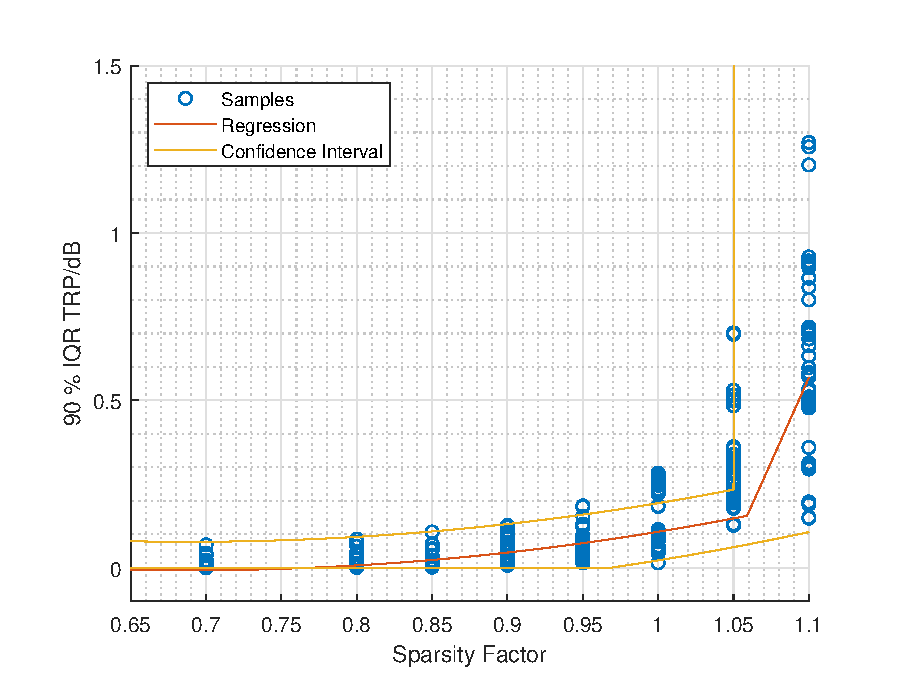
\includegraphics[width=0.49\textwidth]{Matlab/spars-sim7.eps}}
  \centering
  \subfigure[Zoom 2]{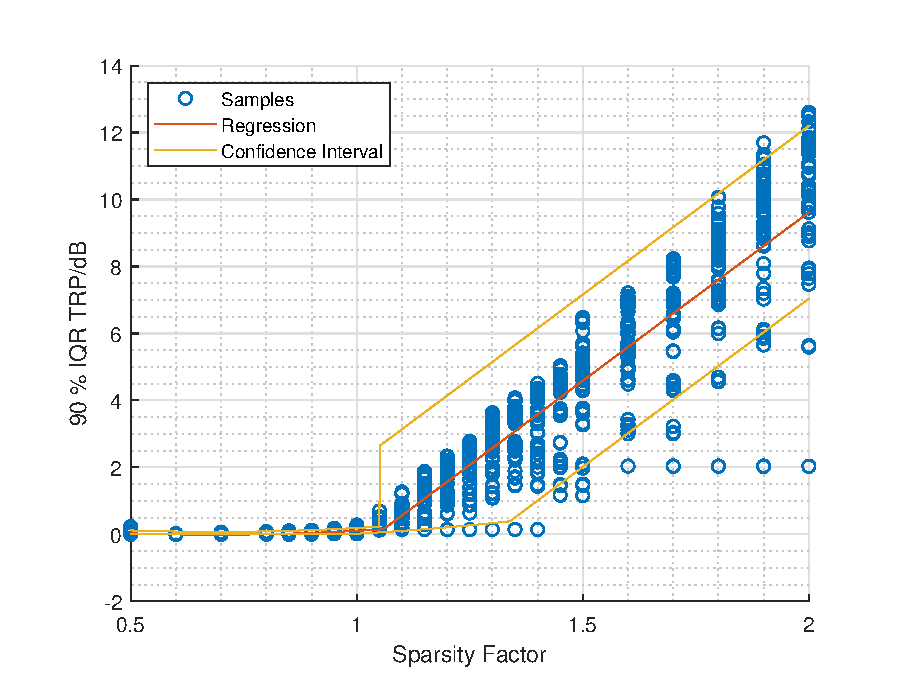
\includegraphics[width=0.49\textwidth]{{Matlab/spars-sim6.eps}}}
\caption{Simulation result over SF}
\label{fig:simressf}
\end{figure}

The marginal probability of the resulting \ac{TRP} \acp{IQR} from the simulation is depicted in fig. \ref{fig:sparssim3}. There are two major areas: Primarily the scattering of the \ac{TRP} is mostly independent of the \ac{SF}. Secondary the \ac{TRP} is dependent from \ac{SF} at around $\text{SF} > 1$. It seems that the \ac{TRP} is mostly independent of all other input parameters.

\subsection{Regression}

The regression of the \ac{TRP} equation is done as described in section \ref{sec:regod} using the parameter matrix $X$ from equation \ref{eq:parammatrix}. The regression is done separately for the two areas. The outcome of the regression is plotted in fig. \ref{fig:simressf} in red.
Starting with $\text{SF}\le 1$. With the parameter matrix $X$, the \ac{COD} is $\SI{48}{\percent}$ and the least significant parameter is the interaction between the array sizes with $p = \SI{47}{\percent}$. In the following both array size parameters are also discarded because of their low significance leading to a \ac{COD} of $\SI{48}{\percent}$, with all parameters significant. So the \ac{CTF} has a slight impact on the resulting regression with a coefficient of $b_3=\SI{3.3e-2}{\decibel}$. This corresponds to the maximum introduced additional error of $b_3\cdot\text{CTF}_\text{max}=b_3\cdot 1$, so the error is negligible. Setting $b_3 = 0$ leads to an \ac{COD} of $\SI{42}{\percent}$.\\
Starting the regression of the second area with $\text{SF} > 1$ also with the parameter matrix $X$ leads to a \ac{COD} of $\SI{92}{\percent}$. There the least significant parameter is the \ac{CTF} with $p = \SI{65}{\percent}$. Further step wise discarding of the least significant parameters leads to a \ac{SF} dependent function with residual dependency to the two-dimensional array size. Discarding the array size gives a \ac{COD} of $\SI{84}{\percent}$. Further discarding of the quadratic \ac{SF} parameter has not a big impact and the \ac{COD} is unchanged. The resulting function is thus

\begin{equation}
\text{TMP}\left(\text{SF}\right)=\begin{cases} 
\SI{0.56}{\decibel}-\SI{1.6}{\decibel}\cdot \text{SF}+\SI{1.2}{\decibel}\cdot\text{SF}^2 & \text{for}\ \text{SF}\le 1.1\\
\SI{-10}{\decibel}+\SI{10}{\decibel}\cdot\text{SF} & \text{for}\ \text{SF}>1.1\end{cases}\,.
\end{equation}

Because of the high scattering level of the second part of the \ac{SF} value range regression, the first part is taken. There it has been proved by regression, that the array size is insignificant. This proves, that the \ac{CrefA} approach is working. 
Furthermore, it has been shown that the \ac{CTF} has a very little impact on the measurement error and can thereby be neglected, so that with the \ac{CTF} the number of measurement points can be effectively reduced. 
Also in the second area, the \ac{CTF} and the array dimensions are mainly insignificant, which is intended. These findings are also proofed by the marginal probabilities plotted in the annex in the figures \ref{fig:sparssim3} and \ref{fig:sparssimbox}.\\
The marginal probability of the means of each scattering for all parameter combination is plotted in fig. \ref{fig:sparssimboxmean}. The mean of the scatterings of the \ac{TRP} is, for $\text{SF} \le 1$, distributed around zero and the value range is always in the vicinity of some $\SI{1e-3}{\decibel}$.\\
The $\SI{95}{\percent}$ confidence interval of the regression is plotted in fig. \ref{fig:simressf} in yellow. It is computed as described in equation \ref{eq:conv}. It is also split in two parts.

\subsection{Comparison of Different Reference Angles}

The same simulation is carried out by using the reference angle introduced by \cite{hansen} in equation \ref{eq:refahansen}. The resulting marginal probability distribution is plotted in fig. \ref{fig:sparssimboxhansen}. Because of the tendentially smaller sampling interval, refer to fig. \ref{fig:evolvpattern3}, the \ac{IQR} of the \ac{TRP} distributions is lower. This leads to an unnecessary high sampling density. Also, the regression parameters show that a residual dependency is present, combined with a lower coefficient of determination as in the \ac{CrefA} sampling density approach from above:\\
For $\text{SF}\le 1$, starting with the regression from equation \ref{eq:parammatrix}, the significant parameters are the \ac{CTF}, the number of elements in $y$ and the \ac{SF} with a \ac{COD} of $\SI{24}{\percent}$. Discarding all parameters except the \ac{CTF} leads to a \ac{COD} of $\SI{21}{\percent}$, so the \ac{TRP} \ac{IQR} is mainly independent of \ac{SF}.\\
For $\text{SF}\ge 1$, starting with the regression from equation \ref{eq:parammatrix}, the significant parameters are the number of elements in $y$, the number of elements in $z$ and the \ac{SF} with a \ac{COD} of $\SI{71}{\percent}$. Discarding the array size parameters leads to a \ac{COD} of $\SI{54}{\percent}$, showing the significant residual correlation between array size and \ac{TRP} \ac{IQR}.\\
A similar outcome is recognized using the reference angle from \cite{2018arXiv180310993F}, where the reference angle increment is computed by formula \ref{eq:hansenrefa}.
To generate the sampling angle the reference angle is multiplied by \ac{SF} and it is provided that the resulting angle increment is less than $\SI{15}{\degree}$.
This results for small arrays in unnecessary fine sampling.
Regarding fig. \ref{fig:sparssimboxericsson}, showing that for small arrays the \ac{IQR} scattering is independently low. That can also be proofed by regression. For $\text{SF}\ge 1$ the significant parameters are the numbers of elements in $z$ and the area of the array with a \ac{COD} of $\SI{73}{\percent}$. Discarding the array size parameters leads to a \ac{COD} of $\SI{44}{\percent}$, whereby the \ac{COD} is with \ac{CrefA} implementation $\SI{84}{\percent}$.

\subsection{Comparison of CSSG and CDG}

\begin{figure}[h]
\centering
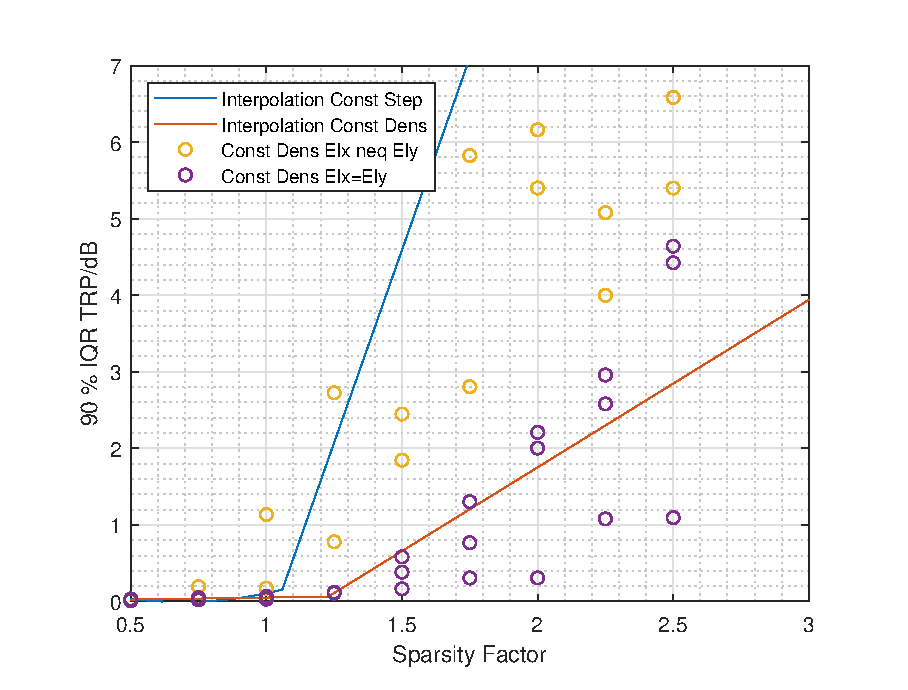
\includegraphics[width=0.49\textwidth]{Matlab/spars-sim3.eps}
\caption{The CDG compared to the CSSG}
\label{fig:cdg}
\end{figure}

The computational effort to simulate the \acp{CDG} is with this implementation very high, caused by the fine $\SI{0.2}{\degree}$ sampling grid.
Therefore, less samples are computed. The result is depicted in fig. \ref{fig:cdg}. It is shown, that for uniform arrays, the performance of the \ac{CDG} is better than the \ac{CSSG}. For non-uniform arrays the performance is equal to a \ac{CSSG}.
This is caused, e.g. for a non-quadratic array, by unnecessary high sampling density in azimuth and sparse sampling in elevation caused by the non-adaptive \ac{CDG}. This leads for the same number of points to a similar or worse result. In addition, using the \ac{CTF}, the number of measurement points is even lower for the \ac{CSSG}.



